\documentclass[10pt,letterpaper]{article}
\usepackage[top=0.85in,left=1.25in,footskip=0.75in,marginparwidth=2in]{geometry}

% use Unicode characters - try changing the option if you run into troubles with special characters (e.g. umlauts)
\usepackage[utf8]{inputenc}

% clean citations
\usepackage{cite}

% hyperref makes references clicky. use \url{www.example.com} or \href{www.example.com}{description} to add a clicky url
\usepackage{nameref,hyperref}

% line numbers
\usepackage[right]{lineno}

% improves typesetting in LaTeX
\usepackage{microtype}
\DisableLigatures[f]{encoding = *, family = * }

% text layout - change as needed
\raggedright
\setlength{\parindent}{0.5cm}
\textwidth 6.25in
\textheight 8.75in

% Remove % for double line spacing
%\usepackage{setspace} 
%\doublespacing

% use adjustwidth environment to exceed text width (see examples in text)
\usepackage{changepage}

% adjust caption style
\usepackage[aboveskip=1pt,labelfont=bf,labelsep=period,singlelinecheck=off]{caption}

% remove brackets from references
\makeatletter
\renewcommand{\@biblabel}[1]{\quad#1.}
\makeatother

% headrule, footrule and page numbers
\usepackage{lastpage,fancyhdr,graphicx}
\usepackage{epstopdf}
\pagestyle{myheadings}
\pagestyle{fancy}
\fancyhf{}
\rfoot{\thepage/\pageref{LastPage}}
\renewcommand{\footrule}{\hrule height 2pt \vspace{2mm}}
\fancyheadoffset[L]{2.25in}
\fancyfootoffset[L]{2.25in}

% use \textcolor{color}{text} for colored text (e.g. highlight to-do areas)
\usepackage{color}

% define custom colors (this one is for figure captions)
\definecolor{Gray}{gray}{.25}

% this is required to include graphics
\usepackage{graphicx}

%
%\usepackage{biblatex}
\usepackage{amsmath}
\usepackage{amssymb}
\usepackage{namedtensor}
\usepackage[version=4]{mhchem}
\usepackage{siunitx}
\usepackage{comment}
\usepackage{mathtools}
\usepackage{xparse,mathtools}
\usepackage{tikz}
\usepackage{booktabs}
\usepackage{footnote}
\makesavenoteenv{tabular}
\makesavenoteenv{table}
\usetikzlibrary{bayesnet}
\usepackage{algorithm}
\usepackage{algpseudocode}
\DeclareSIUnit\Molar{M}
\DeclareMathOperator*{\argmax}{argmax}
\DeclareMathOperator*{\argmin}{arg\,min}

% document begins here
\begin{document}
\vspace*{0.35in}

% title goes here:
\begin{flushleft}
{\Large
\textbf\newline{Bayesian analysis of single molecule fluorescence  colocalization images}
\textbf\newline{Bayesian classification of single molecule fluorescence colocalization images}
}
\newline
% authors go here:
\\
Yerdos A. Ordabayev\textsuperscript{1},
Larry Friedman\textsuperscript{1},
Jeff Gelles\textsuperscript{1,*},
Douglas L. Theobald\textsuperscript{1,*}
\\
\bigskip
\bf{1} Brandeis University
\\
\bigskip
* gelles@brandeis.edu
* dtheobald@brandeis.edu

%possible reviewers to think about:
%Jan-Willem de Meent, Northeastern
%Chris Wiggins, Columbia
%Steve Presse, Arizona State
%Carlas Smith, TU Delft

\end{flushleft}

%\section*{Abstract}
%Multi-wavelength single-molecule fluorescence colocalization methods allow elucidation of complex biochemical reaction mechanisms. However, analysis of colocalization data is an intrinsically challenging and time-consuming problem for multiple reasons. First, to minimize dye photobleaching, images frequently are collected at low signal-to-noise ratios, making it challenging to discriminate real fluorescent spots from noise. Second, transient non-specific interactions of the binder molecule with the surface of the microscope slide can give rise to both false-positive and false-negative detection. Third, current analysis methods require subjective choice of user-set thresholds for such spot parameters as amplitude, diameter and proximity. To overcome these difficulties, we developed a new analysis method based on statistical modeling of the image data. This method: 1) maximizes extraction of useful information from data by analyzing 2-D images, not integrated intensity; 2) discriminates authentic fluorescence spots from fluctuations in background fluorescence in a probabilistic manner and assigns spot probabilities (not merely a binary "spot/no spot" classification); 3) uses a realistic pixel intensity model that accounts for background, spot, and camera noise sources; 4) explicitly models non-specific interactions of binder molecules with the slide surface; and 5) can globally fit data from experimental samples together with negative controls that lack target molecules. The software is implemented in the Python-based Pyro probabilistic programming language which allows easy substitution of different statistical models, efficiently uses parallelized processing (GPU) hardware, and is scalable to large data sets. The algorithm is effective without manual parameter tweaking on both simulated and experiment-derived data sets with a wide range of signal, noise, and non-specific binding characteristics. We anticipate that this work will increase the accessibility and utility of single-molecule fluorescence colocalization methods.

% now start line numbers
\linenumbers

% wc 1220
\section*{Introduction}

%Nature Methods says: To enhance the practical relevance of each paper, description of the method must be accompanied by its validation, its application to an important biological question and results illustrating its performance in comparison to available approaches. Articles are selected for publication that present broad interest, thorough assessments of methodological performance and comprehensive technical descriptions that facilitate immediate application.

A central concern of modern biology is understanding at the molecular level the chemical and physical mechanisms by which protein and nucleic acid macromolecules  perform essential cellular functions.  The operation of many such macromolecules requires that they work not as isolated molecules in solution but as components of dynamic molecular complexes that self-assemble and change structure and composition as they function.  For more than  two decades, scientists have successfully explored the molecular mechanisms of many such complex and dynamic systems using multi-wavelength single molecule fluorescence methods such as smFRET (single-molecule fluorescence resonance energy transfer) \cite{Roy2008-fo} and single-molecule colocalization methods like CoSMoS (colocalization single molecule spectroscopy) \cite{Larson2014-os, Van_Oijen2011-ig}.

CoSMoS is a technique to measure the kinetics of dynamic interactions between individual molecules.  The CoSMoS method has been used for elucidating the mechanisms of complex biochemical processes \textit{in vitro}. Examples include cell cycle regulation \cite{Lu2015-eu}, ubiquitination and proteasome-mediated protein degradation \cite{Lu2015-jq}, DNA replication \cite{Geertsema2014-bt,Ticau2015-ib}, transcription \cite{Zhang2012-no,Friedman2012-if,Friedman2013-sf}, micro-RNA regulation \cite{Salomon2015-kq}, pre-mRNA splicing \cite{Shcherbakova2013-bi, Krishnan2013-fy, Warnasooriya2014-ls}, ribosome assembly \cite{Kim2014-zc}, translation \cite{Wang2015-tt,Tsai2014-mi,OLeary2013-wo}, signal recognition particle-nascent protein interaction \cite{Noriega2014-vj}, and cytoskeletal regulation \cite{Smith2013-qj,Breitsprecher2012-mj}. 

Fig. 1a illustrates an example CoSMoS experiment to measure the interaction kinetics of RNA polymerase molecules with DNA. In the experiment \cite{Rosen2020-zn}, we first measured the locations of individual DNA molecules (the ``targets'') tethered to the surface of an observation chamber at low density. Next, a solution containing RNA polymerase II molecules (the ``binders'') was added to the solution over the surface and the chamber surface was imaged by TIRF (total internal reflection fluorescence) microscopy. When the binder molecules are freely diffusing in solution, they are not visible in TIRF. In contrast, when bound to a target, a single binder molecule is detected as a discrete fluorescent spot colocalized with the target position \cite{Friedman2006-kb, Friedman2015-nx}.

Effective data analysis is a major challenge in the use of the CoSMoS technique. The basic goal is to acquire information at each time point about whether a binder molecule fluorescence spot is observed at the image position of a target molecule (e.g., whether a colocalized green RNA polymerase is observed at the surface location of a blue DNA spot in Fig. 1b). Although CoSMoS images are conceptually simple -- they consist only of diffraction-limited fluorescent spots collected in several wavelength channels -- efficient analysis of the images is inherently challenging. The number of photons emitted by a single fluorophore is limited by fluorophore photobleaching. Consequently, it is desirable to work at the lowest feasible excitation power in order to maximize the duration of experimental recordings and to efficiently capture relevant reaction events. Achieving higher time resolution divides the number of emitted photons between a larger number of images, so that photon shot noise ordinarily dominates the data statistics. Furthermore, the required concentrations of binder molecules can sometimes create significant background noise \cite{Peng2018-ge, Van_Oijen2011-ig}, even with zero-mode waveguide instruments \cite{Chen2014-jd}. These technical difficulties result in CoSMoS images that frequently have low signal-to-noise ratios (SNR), making discrimination of real fluorescent spots from noise a significant challenge. Also, there are usually non-specific interactions of the binder molecule with the chamber surface, and these artefacts can give rise to both false positive and false negative spot detection. These defects in analyzing spot colocalization interfere with the interpretation of CoSMoS data to measure reaction thermodynamics and kinetics and to infer molecular mechanisms.

Most CoSMoS spot detection methods are based on integrating the binder fluorescence intensity over small regions of the image  centered on the location of individual target molecules, and then using crossings of an intensity threshold to score binder molecule arrival and departure \cite{Friedman2015-nx}. However, integration discards data about the spatial distribution of intensity that can (and should) be used to distinguish authentic on-target spots from artefacts caused by noise or off-target binding.  More recently, improved methods \cite{Friedman2015-nx,Smith2019-yb} were developed that directly analyze TIRF images, using the spatial distribution of binder fluorescence intensity around the target molecule location. All of these methods, whether image- or integrated intensity-based, make a binary decision about the presence or absence of a binder spot at the target location.  Treating all binary decisions as equal neglects differences in the confidence of each spot detection decision caused by variations in noise, signal intensity, and non-specific binding.  Failure to account for spot confidence decreases the reliability of downstream thermodynamic and kinetic analysis.

In this paper, we describe a qualitatively different method for analysis of CoSMoS data implemented in a computer program, Tapqir (Kazakh: clever or inventive; pronunciation: \emph{tap-keer}). Tapqir analyzes 2-D image data, not integrated intensities.  Unlike prior methods, our approach is based on an explicit, global model for CoSMoS image formation and uses Bayesian inference to determine the values of model parameters and their associated uncertainties. The model includes realistic shot noise in fluorescent spots and background, camera noise, the size and shape of spots, and the presence of both target-specific and nonspecific binder molecules in the images. Most importantly, instead of yielding a binary spot-/no-spot determination, the algorithm calculates the probability of a target-specific spot being present at each time point and target location. The calculated probability can then be used in subsequent analyses of the molecular thermodynamics and kinetics. Unlike alternative approaches, Tapqir does not use subjective threshold settings so it can be used effectively and accurately by non-expert practitioners. The program is implemented in the Python-based probabilistic programming language Pyro \cite{Bingham2019-qy}, which facilitates modification of the global model and efficient use of graphics processing unit (GPU)-based hardware for rapid parallel processing of data. 

% wc 1300
\section{Results}

\subsection{The Model}

In this work, we present a probabilistic generative model for single-molecule image-data and describe Bayesian inference approach used to obtain posterior distributions of latent model parameters. The generative model can be interpreted as a causal process that produces the observed image data. The graphical model in Figure 2A visually describes latent variables of the model and conditional independence structure of the model. We model the observed image as ``spot'' images of binder molecules superimposed on background image. Fluorescence spots are modeled as a 2D Gaussians parameterized by a set of variables ($h, w, x, y$) which accurately approximates fluorescence microscope point spread function \cite{Zhang2007-rb}. The model depends on various unobserved physical parameters such as background photon intensity and the number, position, shape, and intensity of each spot in the image. The unobserved parameters, in turn, are described by prior distributions which embed into the model our existing knowledge of the experiment, such as the likely position of an on-target spot. Explicitly model on-target and off-target spots.

Our model assumes that at maximum 2 spots in total can be present in a single image and at maximum only one on-target spot. The image model described above allows to capture many of the characteristics of real experimental data, such as site and time dependent fluctuations in the local background signal, time dependent fluctuations in the spot intensity and its position, simultaneous binding of on-target and off-target spots, Gamma distributed noise, which is more realistic than Gaussian noise. Figure 2B,C,D shows examples where there is no spot, one spot, or two spots and corresponding spot parameters in the table.

Total observed intensity is the sum of the offset signal (dark current) plus the photon counts amplified by the gain setting of the camera. The linear relationship between the noise variance and the mean intensity is built into the intensity model through the gain and offset parameters and the gain parameter is fitted along with other parameters. Distribution of the offset signal is obtained as a histogram density signal from the single-molecule images (Figure ).  In Figure we show raw images and their intensity distributions along with the images simulated from the posterior distribution (posterior predictive checking). Comparison of images and distributions for spot/no spot cases show that our model accurately models intensity as a function of mean intensity reflecting the dependence of the noise on the mean intensity. Additionally, Figure shows that the gain parameter is accurately inferred for a simulated set of data with varying gain parameter where the true value of the gain parameter is known.

\subsection{Bayesian Inference and Implementation}

Posterior distributions of latent variables conditioned on the observed data is given by the Bayes' theorem. The evidence in general is intractable. Here we use stochastic variational inference (SVI) approach and maximize the evidence-lower bound (ELBO). Our program Tapqir is open-source (github link) and is implemented in the probabilistic programming language Pyro. The advantage of using PPL like Pyro is its black box SVI approach which allows to focus on the model, efficient computation on GPU, scalability to large datasets. Details of the generative model and variational model are given in the online Methods section.

\subsection{Analysis of simulated data}

As a validation of our model we demonstrate its application to simulated synthetic data. Fake-data simulation is important because it allows to directly check that the inference on latent variables is reliable. Thus, fake-data simulation provides an upper bound of what can be learned reliably about the model for various types of data. Simulation parameters details are described in the online Methods. We made 10 randomized simulations and then fit the synthetic data to the model. Figure 3 shows plots of the simulated values of the global parameters (gain, average on-target spot probability, average off-target spot probability, proximity) vs the fitted values. The results demonstrate that model parameters can be reliably recovered which is good.

MCC plot. Example traces.

\subsection{Analysis of experimental data}

Thermodynamic Analysis.

In this section, we describe different aspects of our model. The Bayesian model described here is holistic in a sense that the observed data and all of the model parameters are interconnected. However, its modular structure allows to view and analyze different parts of the model separately. Below we review briefly the CoSMoS method and the type of data generated by CoSMoS experiments, and then describe the image model, the intensity model, spot-detection, and co-localization aspects of the model.

\subsection{Multi-wavelength single-molecule co-localization methods}

Before describing the approach used for the analysis of CoSMoS data, it is helpful to  review briefly the experimental method. The key features of a CoSMoS experiment include: 1) One species of fluorescently labeled molecule (called the “target”) is tethered to the surface of the observation chamber. Target molecules are immobilized at a surface density sufficiently low that the mean nearest-neighbor distance is large relative to the point-spread function (i.e., the diffraction-limited spot size) of the microscope. 2) Molecules, each species labeled with a different dye color, are added to the solution over the surface, typically at concentrations $\leq 1 \mu$M. When these “binder” molecules are freely diffusing in solution, they are invisible in TIRF. In contrast, when they are bound to the target, single binder molecules are detected as discrete fluorescent spots (Figure \ref{fig:cosmos_experiment}). The combination of features 1 and 2 means that formation of an individual binder-target complex is detected as spot appearance; dissociation of a binder-target complex is detected as spot disappearance \cite{Friedman2006-kb, Friedman2015-nx}.

\subsection{CoSMoS image data}

CoSMoS data analysis requires identifying the locations of target molecules and the corresponding positions in the binder molecule camera channel. Image pre-processing steps include alignment of images from multiple wavelength channels and drift correction \cite{Friedman2015-nx, Smith2019-yb}. Single-molecule images after pre-processing steps consists of a $P \times P$ matrix of pixel intensities with the target molecule at the center of the image. One experiment typically consists of a set of images where we have $N$ target sites ($n \in \{1,\dots,N\}$) each consisting of a series of $F$ different images in a recording ($f \in \{1,\dots,F\}$) (a “recording”).

CoSMoS images consist of offset signal, background intensity and diffraction-limited spots. Detection of on-target binding depends on the intensity of the spot and its distance to the target molecule. The size $P=14$ of the selected area is chosen to be large enough to detect the on-target spot and reliably determine the local background intensity. In addition to the on-target spot, non-specifically bound binder molecules can also be present in the image. Usually no more than two spots are present in the single image. Frequently, identification of on-target binding is complicated by molecules binding off-target which distort the shape of the on-target spot and its apparent distance to the target. 

%\begin{figure}
%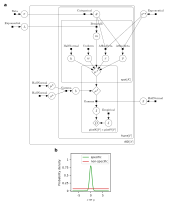
\includegraphics[width=\linewidth]{figures/figure1.jpg}
%\caption{Co-localization single molecule spectroscopy experiment. (A) Target molecules are localized in the blue channel and then on-target and off-target areas of interest are selected. (B) Movies of the binder molecule collected in the green channel. In selected AoI binder molecules can be on-target, off-target, or absent.}
%\label{fig:cosmos_experiment}
%% If the optional argument in the square brackets is "none", then the caption *will not appear in the main figure at all* and only the full caption will appear under the supplementary figure at the end of the manuscript.
%\figsupp[Shorter caption for main text.]{This is a supplementary figure's full caption, which will be used at the end of the manuscript.}{\includegraphics[width=6cm]{frog}}\label{figsupp:sf1}
%\figsupp{This is another supplementary figure.}{\includegraphics[width=6cm]{frog}}
%\figdata{This is a description of a data source.}\label{figdata:first}
%\figdata{This is another description of a data source.}\label{figdata:second}
%\end{figure}

%\begin{figure}
%\includegraphics[width=\linewidth]{figures/figure3a.png}
%\includegraphics[width=\linewidth]{figures/figure3b.png}
%\includegraphics[width=\linewidth]{figures/figure3c.png}
%\caption{Co-localization single molecule spectroscopy experiment. (A) Target molecules are localized in the blue channel and then on-target and off-target areas of interest are selected. (B) Movies of the binder molecule collected in the green channel. In selected AoI binder molecules can be on-target, off-target, or absent.}
%\label{fig:view}
%\end{figure}

\subsection{Image Model Module} 

We model the observed image as ``spot'' images of binder molecules superimposed on background image. In particular, background image consists only of constant background intensity $\mathrm{b}_{nf}$ that can vary from image to image. Our model assumes that at maximum $K=2$ number of spots can be present in a single image.  Fluorescence spot is modeled as a 2D Gaussian which accurately approximates fluorescence microscope point spread function \cite{Zhang2007-rb}. Each spot is parameterized by integrated scalar intensity $\mathrm{h}_{nfk}$, width $\mathrm{w}_{nfk}$, and relative position $\mathrm{x}_{nfk}$ and $\mathrm{y}_{nfk}$ to the target molecule. All of the spot parameters are local/individual for each spot.

We use binary indicator variable $\mathbf{m} = \{\mathrm{m}_{nfk}\}$ to denote the presence of each individual spot ($k \in \{1,\dots,K\}$). The value of the index variable $\theta_{nf} \in \{0,1,\dots,K\}$ specifies the index of the on-target spot when it is present and equals zero when the on-target spot is absent. There are $2^K + K2^{K-1}$ unique combinations of $\mathrm{m}$ and $\theta$ which define the state space for each image. Table~\ref{tab:states} shows the state space when $K=2$. Thus, we get the image model ($\mu^I_{nfij}$) calculated as the sum of the background intensity ($\mathrm{b}_{nf}$) and 2D Gaussian spots ($\mu^S_{knfij}$) present in the image.

\subsection{Spot Detection}

WIP

Spot detection is performed in a probabilistic manner. Spot existence probability depends on the information in the entire image. However, it primarily correlates with the intensity of the spot. Discrimination of spots from random fluctuations in the background signal depends on the prior and not on the threshold parameter. In the absence of prior information uninformative prior can be used. Plotting results show that with half normal prior spots have to be roughly above 1 SNR.

\subsection{Co-localization}

For the spots that are present in the image they can be further classified as on-target (co-localization) or off-target (non-specific). The probability of being on-target or off-target is dictated primarily by the distance to the target. Spots bound on-target and off-target have different prior distributions of their location relative to the target molecule. This prior knowledge is used to discriminate between on- and off-target spots in a probabilistic manner using mixture distributions model. Off-target spots have a uniform prior distribution across the image and can bind anywhere on the surface with equal probability. On-target spots, on the other hand, are clustered near the target molecule. Standard deviation of the distribution of on-target spots depends on the spot localization accuracy and the mapping accuracy between target and binder channels (?). By analyzing simulated data we have established that this parameter, also called the proximity parameter, can be reliably determined by floating it during the fit (Figure ). Alternatively, proximity parameter can be determined experimentally and fixed in the model. Figure show the distribution of the center of mass of on-target spots which are tightly clustered around the target molecule. On the other hand, off-target spots are distributed more uniformly across the area of the image.

Second, the posterior probabilities of being classified as on-target or off-target spot depends on the prior average frequencies of on-target and off-target spots. Increasing the ratio of the off-target molecules to on-target molecules decreases the probability of the spot being on-target reflecting the fact that.

This standard distribution can be determined independently and used as a fixed parameter in the model. However, it can also be floated in the fit and determined from the overall distribution of the center of masses of spots. $\sigma^{xy}$, $\pi^z$, and $\lambda^j$ are correlated. Figure shows simulated data with varying parameters where the true values of parameters are inferred correctly. Note that the posterior probability of the spot class depends on its relative position to the target and average probabilities of on-target and off-target spots.

\subsection{Informal Kinetic/Thermodynamic Analysis}

WIP

% wc
\section{Discussion}

\lipsum[9]

%\section{Methods}

\begin{comment}
\subsection{Approach}

\subsubsection{Probabilistic modeling based on fundamental statistical analysis of data and priors}

To solve the problems with existing CoSMoS data analysis methods identified above, we have developed a new image-analysis-based approach that is accurate, objective, and built on a rigorous statistical approach to the CoSMoS image analysis problem. This method is based on probabilistic modeling methodology. Bayesian model is a statistical model where probability is used to represent all uncertainty within the model, both for observed and hidden quantities in a system of interest. Bayes' theorem allows to perform inference on hidden variables given the observed data. The method described here is time-independent meaning that we ignore the time dimension of the recording -- the order of the images is arbitrary and does not affect the model, as each image is considered statistically independent of the others. We note that this time-independent method can naturally be extended into a time-dependent approach to both more accurately analyze the images and to directly obtain information about molecular kinetic mechanisms.  The proposed methods will eliminate the need for subjective image inspection and minimize the manual work required for CoSMoS data analysis. 

Unlike standard analysis methods for CoSMoS and single molecule FRET (smFRET), which are based on scalar intensity measurements derived from integration of emission in image regions of interest, our model fully uses information contained in the raw two-dimensional microscope images. The value of image data is proven in previous studies \citep{Friedman2015-nx,Smith2019-yb}. To analyze the CoSMoS image classification problem within a Bayesian framework, one must define ideal image shapes for each class (image model) and choose a likelihood function for the observed data (noise model).
\end{comment}

The images are diffraction-limited point spread functions. CoSMoS images consist of background intensity and diffraction-limited spots. The CoSMoS data set consists of a set of images where we have $N$ target sites ($n \in \{1,\dots,N\}$) each consisting of a series of $F$ different images in a recording ($f \in \{1,\dots,F\}$) (a “recording”). Each image is represented as a matrix (2D-array) of $P \times P$ pixel intensities ($i,j \in \{1,\dots,P\}$). We denote entire data set as a multi-dimensional array $D$ and the value of a specific pixel intensity as $D_{nfij}$.

Our goal is to extract useful information from the data such as the probability of the presence of the on-target molecule. Our approach is to use statistical modeling. We formulate a generative model that describes how the observed data is produced. Then we make inference on latent variables that describe the physical parameters of the generative model. 

\subsection{Model}

We build a probabilistic model for CoSMoS data by introducing latent variables that explain how the observed data is generated. A graphical model describing the probabilistic relationships in the model is shown in Figure \ref{fig:graph}. In this directed graph, nodes are either random variables (circles) or deterministic functions (diamonds). Related nodes are connected by edges, with an arrow pointing towards the dependent variable. Dashed boxes represent activation of variables. Finally, plates represent replication and specify an index for the repeated variable.

\begin{figure}[ht]
  \begin{center}
    % model_pca2.tex
%
% Copyright (C) 2010,2011 Laura Dietz
% Copyright (C) 2012 Jaakko Luttinen
%
% The MIT License
%
% See LICENSE file for more details.

% PCA model

%\beginpgfgraphicnamed{model-pca}
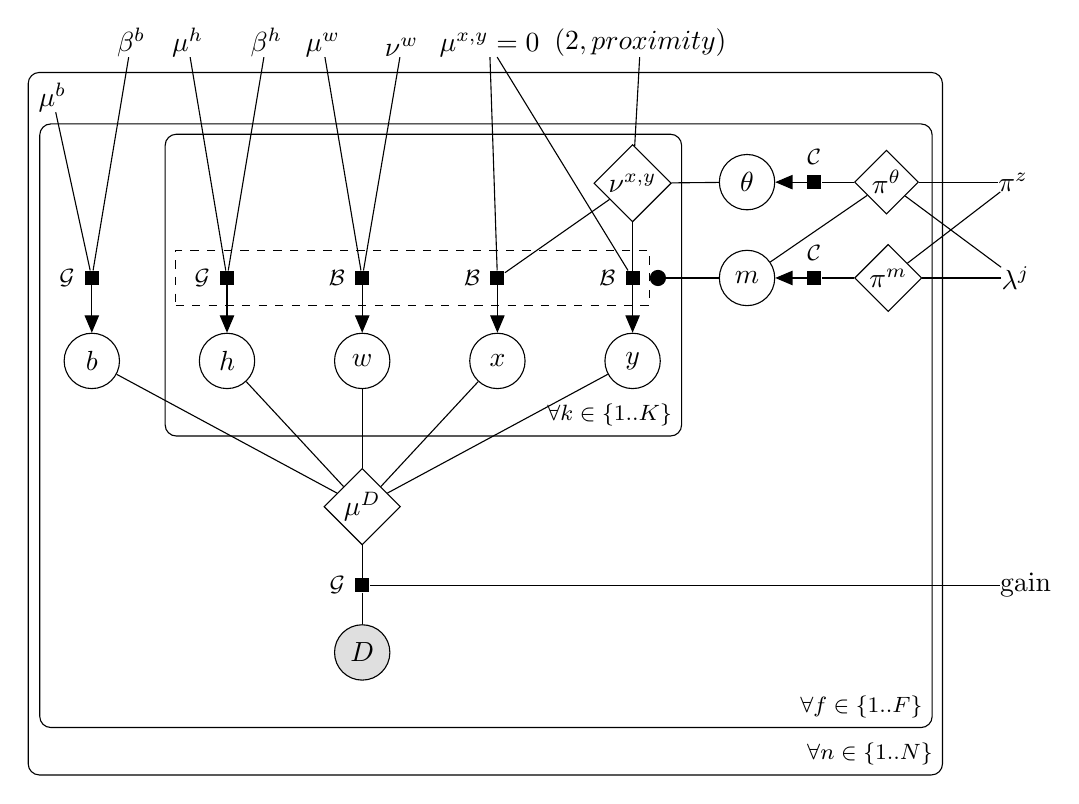
\begin{tikzpicture}

  % Define nodes

  % Y
  \node[obs]          (D)   {$D$}; %

  % W and X
  \node[det, above=of D]            (md) {$\mu^D$} ; % 
  \node[latent, above=of md] (w)   {$w$}; %
  \node[latent, above=of md, left=of w]  (h)   {$h$}; %
  \node[latent, above=of md, left=of h]  (b)   {$b$}; %
  \node[latent, above=of md, right=of w]  (x)   {$x$}; %
  \node[latent, above=of md, right=of x] (y)   {$y$}; %

  % b hyperparameters
  \node[const, above=2.8 of b, xshift=-0.5cm] (mb) {$\mu^b$} ; %
  \node[const, above=3.5 of b, xshift=0.5cm]  (bb) {$\beta^b$} ; %

  % h hyperparameters
  \node[const, above=3.5 of h, xshift=-0.5cm] (mh) {$\mu^h$} ; %
  \node[const, above=3.5 of h, xshift=0.5cm]  (bh) {$\beta^h$} ; %

  % w hyperparameters
  \node[const, above=3.5 of w, xshift=-0.5cm] (mw) {$\mu^w$} ; %
  \node[const, above=3.5 of w, xshift=0.5cm]  (nw) {$\nu^w$} ; %

  % xy hyperparameters
  \node[const, above=3.5 of x, xshift=-0.1cm] (mxy) {$\mu^{x,y}=0$} ; %
  \node[const, above=3.5 of y, xshift=0.1cm] (pr) {$(2,proximity)$} ; %
  \node[det, above=1.4 of y]  (nxy) {$\nu^{x,y}$} ; %

  % Factors
  \factor[above=of D] {D-f} {left:$\mathcal{G}$} {} {} ; %
  \factor[above=0.6 of b] {b-f} {left:$\mathcal{G}$} {mb,bb} {b} ; %
  \factor[above=0.6 of h] {h-f} {left:$\mathcal{G}$} {mh,bh} {h} ; %
  \factor[above=0.6 of w] {w-f} {left:$\mathcal{B}$} {mw,nw} {w} ; %
  \factor[above=0.6 of x] {x-f} {left:$\mathcal{B}$} {mxy,nxy} {x} ; %
  \factor[above=0.6 of y] {y-f} {left:$\mathcal{B}$} {mxy,nxy} {y} ; %

  % D hyperparameters
  \node[const, right=8 of D-f] (g) {gain} ; %

  % m and theta
  \node[latent, right=of y-f] (m)   {$m$}; %
  \node[latent, above=0.5 of m] (t)   {$\theta$}; %

  % m and theta hyperparameters
  \node[det, right=1. of m]        (pm) {$\pi^m$} ; %
  \node[det, right=1. of t]        (pt) {$\pi^\theta$} ; %
  \node[const, right=of pt] (pz) {$\pi^z$} ; %
  \node[const, right=of pm] (lj) {$\lambda^j$} ; %

  % theta hyperparameters
  %\node[const, right=1.2 of t] (pt) {$\pi^\theta(\pi^z,\lambda^j)$} ; %

  % noise
  %\node[latent, right=2.5cm of y-f]         (t)   {$\tau$}; %
  %\node[const, above=of t, xshift=-0.5cm] (at)  {$\alpha_\tau$} ; %
  %\node[const, above=of t, xshift=0.5cm]  (bt)  {$\beta_\tau$} ; %

  % Factors
  \factor[right=of m] {m-f} {above:$\mathcal{C}$} {pm} {m} ; %
  \factor[right=of t] {t-f} {above:$\mathcal{C}$} {pt} {t} ; %
  %\factor[above=of x] {x-f} {left:$\mathcal{N}$} {mx,ax} {x} ; %
  %\factor[above=of t] {t-f} {left:$\mathcal{G}$} {at,bt} {t} ; %
  %\factoredge {dot,t} {y-f} {y} ; %

  \gate {m-gate} {(h-f)(h-f-caption)(h-f)(h-f-caption)(w-f)(w-f-caption)(x-f)(x-f-caption)(y-f)(y-f-caption)} {m}

  % Connect w and x to the dot node
  \factoredge[-] {g,md} {D-f} {D} ;
  \edge[-] {b,h,w,x,y} {md} ;
  \edge[-] {pz,lj,m} {pt} ;
  \edge[-] {pz,lj} {pm} ;
  \edge[-] {t,pr} {nxy} ;

  % Plates
  \plate {K} { %
    (h)(h-f)(h-f-caption) %
    (w)(w-f)(w-f-caption) %
    (x)(x-f)(x-f-caption) %
    (y)(y-f)(y-f-caption) %
    (m-gate) %
    (nxy)
  } {$\forall k \in \{ 1..K \}$} ;
  \plate {F} { %
    (K)
    (t)(t-f)(t-f-caption)(pt) %
    (m)(m-f)(m-f-caption)(pm) %
    (b)(b-f)(b-f-caption) %
    (md) %
    (D)(D-f)(D-f-caption) %
  } {$\forall f \in \{ 1..F \}$} ;
  \plate {N} { %
    (F)
    (mb)
  } {$\forall n \in \{ 1..N \}$} ;
  %\plate {} {%
    %(y)(y-f)(y-f-caption) %
    %(w)(w-f)(w-f-caption) %
    %(dot) %
    %(yx.north west)(yx.south west) %
  %} {$M$} ;

\end{tikzpicture}
%\endpgfgraphicnamed

%%% Local Variables: 
%%% mode: tex-pdf
%%% TeX-master: "example"
%%% End: 


  \end{center}
  \caption{Graphical model for the Bayesian classification model used in Pyro. The model has a modular structure consisting of three parts: classifier, the spot model, and the noise model. Hidden variables (circles) - background intensity ($b$), integrated intensity of the spot ($h$), width of the spot ($w$), position of the spot on the $x$-axis ($x$) and on the $y$-axis ($y$), existence indicator of spots ($m$), and index of the on-target spot ($\theta$). Observed variable (shaded circle) - image of the area of interest ($D$). Variables nested in plates are repeated for a number of times displayed at the bottom-right corner - target sites ($N$), frame count ($F$), number of spots in a single image ($K$). Densities are depicted as  small filled boxes. Deterministic functions are depicted as diamonds. Constants and hyperparameters are written without any borders. Gate (dashed box) represents variable activation conditioned on another variable.}
  \label{fig:graph}
\end{figure}

\subsubsection{Physical model}

We model the observed image data as ``spot'' images of binder molecules superimposed on background image. In particular, background image consists only of constant background intensity $\mathrm{b}_{nf}$ that can vary from image to image. Our model assumes that at maximum $K$ number of spots can be present in a single image.  Fluorescence spot is modeled as a 2D Gaussian which accurately approximates fluorescence microscope point spread function \citep{Zhang2007-rb}. Each spot is parameterized by integrated scalar intensity $\mathrm{h}_{nfk}$, width $\mathrm{w}_{nfk}$, and positions $\mathrm{x}_{nfk}$ and $\mathrm{y}_{nfk}$ on the image:

\begin{equation}
    \mu^{S}_{nfkij} =
        \dfrac{\mathrm{h}_{nfk}}{2 \pi \mathrm{w}^2_{nfk}} \exp{\left[ -\dfrac{(i-\mathbf{x}_{nfk})^2 + (j-\mathrm{y}_{nfk})^2}{2\mathrm{w}^2_{nfk}} \right]}
\end{equation}

We use binary indicator variable $\mathbf{m} = \{\mathrm{m}_{nfk}\}$ to denote the presence of each individual spot ($k \in \{1,\dots,K\}$). The value of the index variable $\theta_{nf} \in \{0,1,\dots,K\}$ specifies the index of the on-target spot when it is present and equals zero when the on-target spot is absent. There are $2^K + K2^{K-1}$ unique combinations of $\mathrm{m}$ and $\theta$ which define the state space for each image. Table~\ref{tab:states} shows the state space when $K=2$.

Thus, we get the image model ($\mu^I_{nfij}$) calculated as the sum of the background intensity ($\mathrm{b}_{nf}$) and 2D Gaussian spots ($\mu^S_{knfij}$) present in the image:

\begin{equation}
    \mu^\mathrm{I}_{nfij} = \mathrm{b}_{nf} + \sum_{\mathrm{m}_{nfk}=1} \mu^S_{knfij}
\end{equation}

\begin{figure}
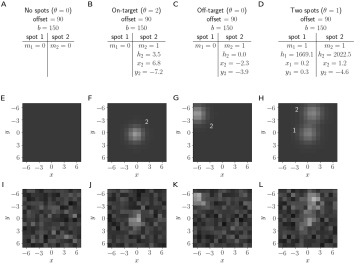
\includegraphics[width=\linewidth]{figures/figure2/figure2.png}
%\includegraphics[width=\linewidth]{figures/figure2g.png}
\caption{Image models. CoSMoS images are modeled as 2D Gaussian spots superimposed onto the background intensity and the offset. Examples of the ideal image shapes for cases when there are (A,E,I) no spots, (B,F,J) single on-target spot, (C,G,K) single off-target spot, and (D,H,L) two spots. Noisy images (I-L) are generated using Gamma distribution with the parameter gain = 7 as described in the text.}
\label{fig:model}
\end{figure}

\subsubsection{Noise model}

\begin{comment}
Shot noise originates from a stochastic nature of photon counting which can be modeled by a Poisson process. The number of photons that fall on each pixel of the camera is Poisson distributed where the variance of the signal equals the mean value of the signal. Gain is a camera setting that amplifies the signal from camera sensors. Our model uses Gamma distribution parameterized by mean intensity ($\mu^D_{nfij}$) and gain ($g$) to model the linear relationship between the expected value of the signal and the variance with which the signal scatter about its expected value. Figure \ref{fig:model}  shows images  where the ideal images were perturbed with Gamma noise for no-spot (D), single spot (E), and two spots (F) images.
\end{comment}

Observed images are contaminated by noise. Noise is a stochastic phenomenon and therefore is described by the likelihood function. The likelihood describes the probability of the observed image given the image model. Scatter about the expected value of signal intensity ($\mu^I_{nfij}$) is determined by photon shot noise and the camera gain that amplifies the signal. We use Gamma distribution as a noise model which is more flexible than Gaussian noise and can better approximate Poissonian camera noise. In addition, there is a noise in the offset signal. Its distribution can be obtained from the camera images:

\begin{equation}
    I_{nfij} \sim \textbf{Gamma} (\mu^I_{nfij}, \sqrt{\mu^I_{nfij} \gamma})
\end{equation}

\begin{equation}
    \delta_{nfij} \sim \textbf{Categorical}_{\{ \delta_r \}^R_{r=1}}(\bm{\pi}^\delta)
\end{equation}

\begin{equation}
    D_{nfij} = \delta_{nfij} + I_{nfij}
\end{equation}

where $I_{nfij}$ is the signal intensity and $\gamma$ is the gain setting of the camera. $\delta_{nfij}$ is a camera offset and $\bm{\pi}^\delta$ is its distribution that can be obtained empirically from the dark corners of the images.

\subsubsection{Priors}
Prior distribution describe our assumptions about the model. On-target spots have a Bernoulli distribution with average probability $\pi^z$, while the number of off-target spots has a truncated Poisson distribution with the rate parameter $\lambda^j$. For the spot intensity we assume broad range of values given by:

\begin{equation}
    h_{knf} \sim \mathbf{HalfNormal}(\sigma^h)
\end{equation}
 
 Spot width has a uniform prior confined to a range:
 
\begin{equation}
    w_{knf} \sim \textbf{Uniform}(w_{\min}, w_{\max})
\end{equation}

Priors for the position of the spot depends whether the spot is on-target or non-specific. On-target spots are localized around the target molecule within the experimentally determined co-localization accuracy. On the other hand, non-specific binding can occur anywhere within the image and therefore has a uniform distribution across the image:

\begin{equation}
    x_{knf}, y_{knf} \sim
    \begin{cases}
    \textbf{AffineBeta}(0, \nu^{xy}, -\frac{P+1}{2}, \frac{P+1}{2}) & \text{$\theta_{nf} = k$ (on-target)} \\
    \textbf{Uniform}(-\frac{P+1}{2}, \frac{P+1}{2}) & \text{$\theta_{nf} \neq k$ (off-target)}
    \end{cases}
\end{equation}

Due to the irregularity of the filed of view of the microscope we assume separate prior for each target site:

\begin{equation}
    b_{nf} \sim \textbf{Gamma}(\mu^b_n, \sigma^b_n)
\end{equation}

\begin{table}
\caption{\label{tab:states}State space for $K = 2$.}
% Use "S" column identifier to align on decimal point 
\begin{tabular}{c c c c c}
\toprule
state   & first spot $m_{nf1}$ & second spot $m_{nf2}$ & on-target index $\theta_{nf}$  & probability \\
\midrule
$1$       & $0$     & $0$     & $0$         &  \\
$2$       & $1$     & $0$     & $0$         &  \\
$3$       & $0$     & $1$     & $0$         &  \\
$4$       & $1$     & $1$     & $0$         &  \\
$5$       & $\mathbf{1}$    & $0$     & $1$         &  \\
$6$       & $\mathbf{1}$    & $1$     & $1$         &  \\
$7$       & $0$     & $\mathbf{1}$    & $2$         &  \\
$8$       & $1$     & $\mathbf{1}$    & $2$         &  \\
\bottomrule
\end{tabular}
\end{table}

\subsubsection{Joint Distribution}

Factorization of the joint probability of the model is given by:

\begin{equation}
    p_\psi (\mathbf{D}, \mathbf{v})
    = p_\gamma (\mathbf{D} | \mathbf{b}, \mathbf{m}, \mathbf{h}, \mathbf{w}, \mathbf{x}, \mathbf{y})
    p_{\mu^b, \sigma^b} (\mathbf{b})
    p (\mathbf{h})^\mathbf{m}
    p (\mathbf{w})^\mathbf{m}
    p_{\sigma^{\mathrm{xy}}} (\mathbf{x}|\mathbf{\theta})^\mathbf{m}
    p_{\sigma^{\mathrm{xy}}} (\mathbf{y}|\mathbf{\theta})^\mathbf{m}
    p_{\pi^z, \lambda^j} (\mathbf{m}, \theta)
\end{equation} 

where $\psi = \{ \pi^z, \lambda^j, \mu^b, \sigma^b, \gamma \}$ and $\mathbf{v} = \{ \mathbf{b}, \mathbf{m}, \theta, \mathbf{h}, \mathbf{w}, \mathbf{x}, \mathbf{y} \}$.

\subsection{Inference}

The evidence, i.e. probability of the data, is given by:

\begin{equation}
    p_\psi (\mathbf{D}) = \int_\mathbf{v} p_\psi (\mathbf{D}, \mathbf{v}) d\mathbf{v}
\end{equation}

Our goal is to learn good model parameters by maximizing the log evidence:

\begin{equation}
    \psi_{\max} = \argmax_\psi \log p_\psi (\mathbf{D})
\end{equation}

In addition, we want to obtain the posterior over the latent variables $\mathbf{v}$ given the observed data:

\begin{equation}
    p_{\psi_{\max}} (\mathbf{b}, \mathbf{m}, \theta, \mathbf{h}, \mathbf{w}, \mathbf{x}, \mathbf{y}|\mathbf{D}) =
    \dfrac{p_{\psi_{\max}}(\mathbf{D}, \mathbf{b}, \mathbf{m}, \theta, \mathbf{h}, \mathbf{w}, \mathbf{x}, \mathbf{y})}
    {\int_{\mathbf{b}, \mathbf{h}, \mathbf{w}, \mathbf{x}, \mathbf{y}}
    \sum_{\mathbf{m}, \theta}
    p_{\psi_{\max}} (\mathbf{D}, \mathbf{b}, \mathbf{m}, \theta, \mathbf{h}, \mathbf{w}, \mathbf{x}, \mathbf{y})
    d\mathbf{b} d\mathbf{h} d\mathbf{w} d\mathbf{x} d\mathbf{y}}
\end{equation}

\begin{equation}
    p_{\psi_{\max}}(\mathbf{b}, \mathbf{m}, \theta, \mathbf{h}, \mathbf{w}, \mathbf{x}, \mathbf{y}|\mathbf{D})
    \simeq q_{\phi}(\mathbf{b}) q(\mathbf{m}, \theta) q(\mathbf{h})^\mathbf{m}
    q(\mathbf{w})^\mathbf{m} q(\mathbf{x})^\mathbf{m} q(\mathbf{y})^\mathbf{m}
\end{equation}

\subsection{Experimental data}

In this experiment, we labeled the NusG protein with an orange dye. We then tethered to a microscope slide blue-dye-labeled DNA molecules at very low surface density (so that each molecule is resolved as a separate fluorescent spot) and observed real-time binding and dissociation of the other labeled molecules during the transcription process and its regulation. The signal from the orange dye was split between short wavelength and long wavelength channels. The signal in the short wavelength channel was attenuated to varying degree to produce data sets with a range of SNR. Images from the long wavelength channel with high SNR were analyzed to determine "true" identities of the images.

%\subsection{Image analysis, probabilities not binary classification}

%Expresses uncertainty. Allows downstream analysis. 

%\subsection{Flexible framework. Can select and use different models depending on the experiment}

%\subsubsection{Ability to jointly analyze different experimental conditions}

%\subsubsection{Models easily expandable to incorporate other data features}


\clearpage
\newpage
\section*{Figures and figure captions}
\pagebreak

\newgeometry{textheight=9in,textwidth=7.2in}
\renewcommand{\figurename}{Fig.}

% figure 1
\begin{figure}[h]
\centering
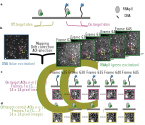
\includegraphics[width=145mm]{figures/figure1/figure1.png}
\caption{\textbf{Example CoSMoS experiment.} Data set A in Extended Data Table 1. \textbf{a}, Experiment schematic. DNA target molecules labeled with a blue-excited fluorescent dye (blue star) are tethered to the microscope slide surface. RNA polymerase II (RNApII) binder molecules labeled with a green-excited dye (green star) are present in solution. \textbf{b}, Data collection and preprocessing. After collecting a single image with blue excitation to identify the location of the DNA molecules, a time sequence of RNApII images were collected with green excitation.  Preprocessing of the images includes mapping of the corresponding points in target and binder channels, drift correction, and identification of two sets of areas of interest (AOIs).  One set corresponds to locations of target molecules (e.g., purple square); the other corresponds to locations where no target is present (e.g., yellow square). \textbf{c}, On-target data. Data are time sequences of $14 \times 14$ pixel AOI images centered at each target molecule. Frames show on-target (e.g., frame 630) and off-target (e.g., frame 645) binding of RNApII molecules. \textbf{d}, Off-target control data. Control data consists of images collected from randomly selected sites at which no target molecule is present. }
\label{fig:cosmos_experiment}
\end{figure}

% figure 2
\begin{figure}[h]
\centering
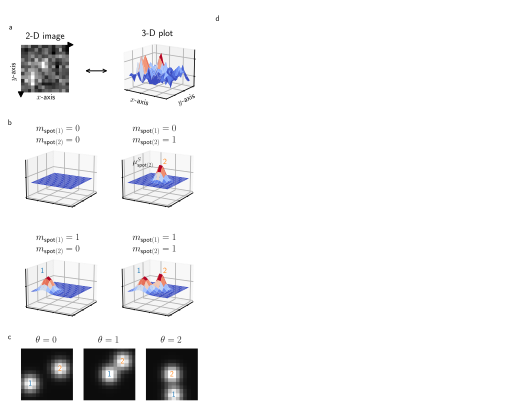
\includegraphics[width=\textwidth]{figures/figure2.png}
\label{fig:tapqir_model}
\caption{\textbf{Depiction of the probabilistic image model and model parameters.} \textbf{a}, Example AOI image from the Rpb1\textsuperscript{SNAP549} experimental data set. The AOI image is a matrix of $14 \times 14$ pixel intensities which is shown here as both a 2-D grayscale image and as a 3-D intensity plot. The image contains two spots, one is centered at target location (image center) and the other is located off-target. \textbf{b}, Examples of four idealized noise-free image representations ($\mu^I$). Image representations consist of zero, one, or two idealized spots ($\mu^S$) superimposed on a constant background ($b$). Each fluorescent spot is represented as a 2-D Gaussian parameterized by integrated intensity ($h$), width ($w$), and position ($x$, $y$). The presence of spots is encoded in the binary spot existence indicator $m$. \textbf{c}, Simulated idealized images illustrating different values of the target-specific spot index parameter $\theta$. $\theta = 0$ corresponds to a case when no specifically bound molecule is present; $\theta = 1$ or 2 corresponds to the cases in which the specifically bound molecule is spot 1 or 2, respectively. \textbf{d}, Condensed graphical representation of the probabilistic model. Model parameters are depicted as circles and deterministic functions as diamonds. Observed image ($D$) is represented by a shaded circle. Related nodes are connected by edges, with an arrow pointing towards the dependent node (e.g., the shape of each 2-D Gaussian spot $\mu^S$ depends on spot parameters $h$, $w$, $x$, and $y$). Plates (rounded rectangles) contain entities that are repeated for the number of instances displayed at the bottom-right corner: number of AOIs ($N$), frame count ($F$), and/or maximum number of spots in a single image ($K=2$). Parameters outside of the plates are global quantities that apply to all frames of all AOIs. A more complete version of the graphical model specifying the relevant probability distributions is given in Extended Data Fig. 1a. }
\end{figure}

% figure 3
\begin{figure}[h]
\centering
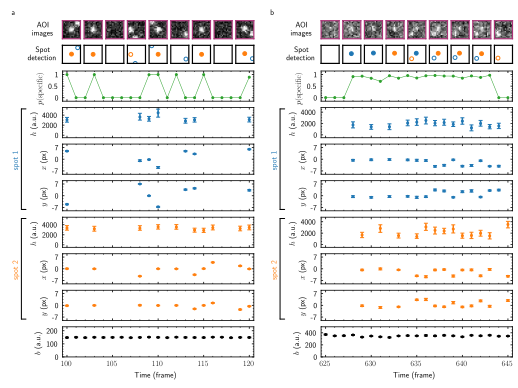
\includegraphics[width=\textwidth]{figures/figure3.png}
\caption{\textbf{Tapqir analysis and inferred model parameters.} \textbf{a},\textbf{b}, Tapqir was applied to simulated data (lamda0.5 parameter set in Supplementary Data 1) (\textbf{a}) and to experimental data (Data set A in Extended Data Table 1) (\textbf{b}). (\textbf{a}) and (\textbf{b}) each show a short extract from a single target location in the corresponding data set. The first row shows AOI images for the subset of frames indicated by gray shaded stripes in the plots. The second row shows the locations of spots determined by Tapqir. Only data for spots with a spot probability $p(m=1) > 0.5$ are shown. Spots predicted to be target-specific ($p(\theta=k)>0.5$ for spot $k$) are shown as filled circles. The graphs show the probability of there being any target-specific spot in a frame ($p(\mathsf{specific})$; green), spot intensity ($h$), location ($x$, $y$) of spot 1 (blue) and spot 2 (orange), and AOI background intensity ($b$). Error bars: 95\% CI (credible interval).  }
\label{fig:tapqir_analysis}
\end{figure}

% figure 4
\begin{figure}[h]
\centering
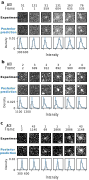
\includegraphics[width=\textwidth]{figures/figure4.png}
\caption{\textbf{Reproduction of experimental data by posterior predictive sampling.} Example frames are shown from Data set A  (\textbf{a}: $\mathrm{SNR}=1.63$), Data set B (\textbf{b}: $\mathrm{SNR}=3.43$), Data set C (\textbf{c}: $\mathrm{SNR}=4.18$), and Data set D (\textbf{d}: $\mathrm{SNR}=4.85$) in Extended Data Table 1. In each panel the top row shows AOI images selected from the experimental data and middle row shows corresponding images simulated by sampling from the posterior distributions. The bottom row shows pixel intensity distributions from the experimental and posterior prediction images shown. }
\label{fig:posterior_samples}
\end{figure}
\clearpage
\newpage

% figure 5
\begin{figure}[h]
\centering
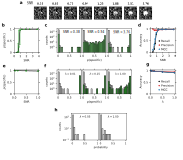
\includegraphics[width=1\textwidth]{figures/figure5.png}
\caption{\textbf{Tapqir performance on simulated data with different SNRs or different non-specific binding rates.} \textbf{a-d}, Analysis of simulated data over a range of SNR. SNR was varied in the simulations by changing spot intensity  $h$ while keeping other parameters constant (Supplementary Data 3). \textbf{a}, Example images showing the appearance of the same target-specific spot simulated with increasing SNR.   \textbf{b}, Mean of Tapqir-calculated target-specific spot probability $p(\mathsf{specific})$ (with 95\% high-density region) for the subset of images where target-specific spots  are known to be present. \textbf{c}, Histograms of $p(\mathsf{specific})$ for selected simulations with SNR indicated. Data are shown as stacked bars for images known to have (green, 15\%) or not have (gray, 85\%) target-specific spots.  Count is zero for bins where bars are not shown. \textbf{d}, Accuracy of Tapqir image classification with respect to presence/absence of a target-specific spot. Accuracy was assessed by MCC, recall, and precision (see Text and Methods). \textbf{e-g}, Same as in (\textbf{b-d}) but for the data simulated over a range of non-specific binding rates $\lambda$ at fixed SNR = 3.76 (Supplementary Data 1). \textbf{h}, Same as in (\textbf{c}) but for the data simulated over a range of non-specific binding rates $\lambda$ with no target-specific binding ($\pi = 0$) (Supplementary Data 4).}
\label{fig:tapqir_performance}
\end{figure}

% figure 6
% move dots in between sample1 2
\begin{figure}[h]
\centering
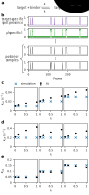
\includegraphics[width=\textwidth]{figures/figure6.png}
\caption{\textbf{Tapqir analysis of association/dissociation kinetics and thermodynamics.} \textbf{a} Chemical scheme for a one-step association/dissociation reaction at equilibrium with apparent first-order binding and dissociation rate constants $k_{\mathrm{on}}$ and $k_{\mathrm{off}}$, respectively. \textbf{b}, A simulation of the reaction in (\textbf{a}) and scheme for kinetic analysis with Tapqir. Simulation used $\mathrm{SNR} = 3.76$, $k_\mathrm{on} = 0.02$ s$^{-1}$, $k_\mathrm{off} = 0.2$ s$^{-1}$, and a high target-nonspecific binding frequency $\lambda = 1$ (Supplementary Data 5, dataset kon0.02lambda1). Full dataset consists of 100 AOI locations and 1000 frames each for on-target data and off-target control data. Shown is a short extract of on-target data from a single location in the simulation.  Plots show simulated presence/absence of the target-specific spot (purple) and Tapqir-calculated estimate of corresponding target-specific spot probability $p(\mathsf{specific})$ (green). One thousand binary traces (e.g., black records) were sampled from the $p(\mathsf{specific})$ posterior distribution and used to infer $k_\mathrm{on}$ and $k_\mathrm{off}$ using a two-state hidden Markov model (HMM) (see Methods). Each sample trace contains well-defined time intervals corresponding to target-specific spot presence and absence (e.g., $\Delta t_\mathrm{on}$ and $\Delta t_\mathrm{off}$). \textbf{c,d,e}, Kinetic and equilibrium constants from simulations (Supplementary Data 5) using a range of $k_\mathrm{on}$ values and  target-nonspecific spot frequencies $\lambda$, with constant $k_\mathrm{off} = 0.2$ s$^{-1}$. \textbf{c} Values of $k_{\mathrm{on}}$ used in simulations (blue) and mean values (and 95\% CIs, black) inferred by HMM analysis from the 2000 posterior samples. \textbf{d}, Same as (\textbf{c}) but for $k_{\mathrm{off}}$. \textbf{e},  Binding equilibrium constants $K_{\mathrm{eq}} = k_{\mathrm{on}} / k_{\mathrm{off}}$ used in simulation (blue) and inferred from Tapqir-calculated $\pi$ as $K_{\mathrm{eq}} = \pi / (1 - \pi)$ (black). }
\label{fig:kinetic_analysis}
\end{figure}
\clearpage
\pagebreak

% figure 7
% add to Methods how CI is calculated
\begin{figure}[h]
\centering
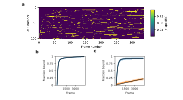
\includegraphics[width=\textwidth]{figures/figure7.png}
\caption{\textbf{Extraction of target-binder association kinetics from example experimental data.} Data are from Data set B (see Extended Data Table 1).  \textbf{a}, Probabilistic rastergram representation of Tapqir-calculated target-specific spot  probabilities $p(\mathsf{specific})$ (color scale). AOIs were ordered by decreasing times-to-first-binding. For clarity, only every thirteenth frame is plotted. \textbf{b}, Time-to-first-binding distribution using Tapqir. Plot shows the cumulative fraction of AOIs that exhibited one or more target-specific binding events by the indicated frame number (green) and fit curve (black). Shading indicates uncertainty. \textbf{c} Time-to-first-binding distribution using an empirical spot-picker method \cite{Friedman2013-sf}. The spot-picker method jointly fits first spots observed in off-target control AOIs (orange) and in on-target AOIs (blue) with fit curves (black). \textbf{d}, Values of kinetic parameters  $k_\mathrm{a}$, $k_\mathrm{ns}$, and $A_\mathrm{f}$ (see text) derived from fits in \textbf{b} and \textbf{c}. Uncertainties reported in (\textbf{b, c, d}) represent 95\% credible intervals for Tapqir and 95\% confidence intervals for spot-picker (see Methods).
}
\label{fig:experimental_data}
\end{figure}

\nolinenumbers

%This is where your bibliography is generated. Make sure that your .bib file is actually called library.bib
\bibliography{references}

%This defines the bibliographies style. Search online for a list of available styles.
\bibliographystyle{abbrv}

\section{Supplementary Material}

\subsection{Variable definitions}

Target site
\begin{equation*}
    n \in \{1,\dots,N\}
\end{equation*}
%
Frame number
\begin{equation*}
    f \in \{1,\dots,F\}
\end{equation*}
%
$x$-axis pixel number
\begin{equation*}
    i \in \{1,\dots,I\}
\end{equation*}
%
$y$-axis pixel number
\begin{equation*}
    j \in \{1,\dots,J\}
\end{equation*}
%
Spot index
\begin{equation*}
    k \in \{1,\dots,K\}
\end{equation*}
%
Background intensity
\begin{equation*}
    b_{nf} > 0
\end{equation*}
%
Hidden state
\begin{equation*}
    m_{nf}
\end{equation*}
%
Integrated spot intensity
\begin{equation*}
    h_{nfk} > 0
\end{equation*}
%
Ideal spot shape
\begin{equation*}
    \mu^{D}_{nfij} = b_{nf} + \sum_k \dfrac{m_{nfk}h_{nfk}}{2 \pi w^2_{nfk}} \exp{\left ( -\dfrac{(i-x_{nfk})^2 + (j-y_{nfk})^2}{2w^2_{nfk}} \right)}
\end{equation*}

\end{document}
